\begin{figure}[p]
\centering
    \begin{subfigure}[t]{0.9\textwidth}
    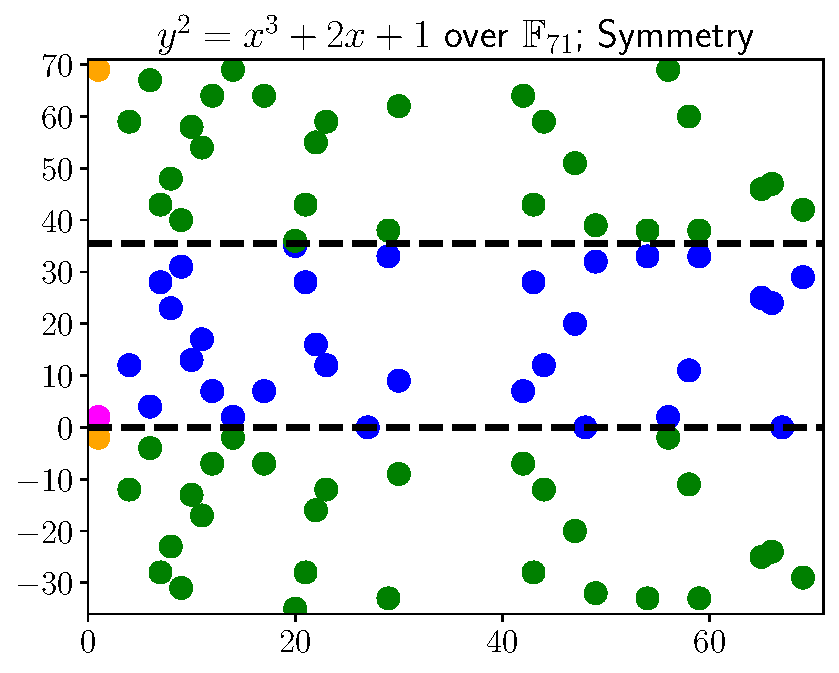
\includegraphics[width=\textwidth]{plots/ec_finite/ec_finite_F_71_2_1_symmetry_base.pdf}
    \caption{Plot with all $y$ values in $\brackets{-p/2,p}$.}
    \label{fig:ec_finite_plots_symmetry_main}
    \end{subfigure}

    \begin{subfigure}[t]{0.45\textwidth}
    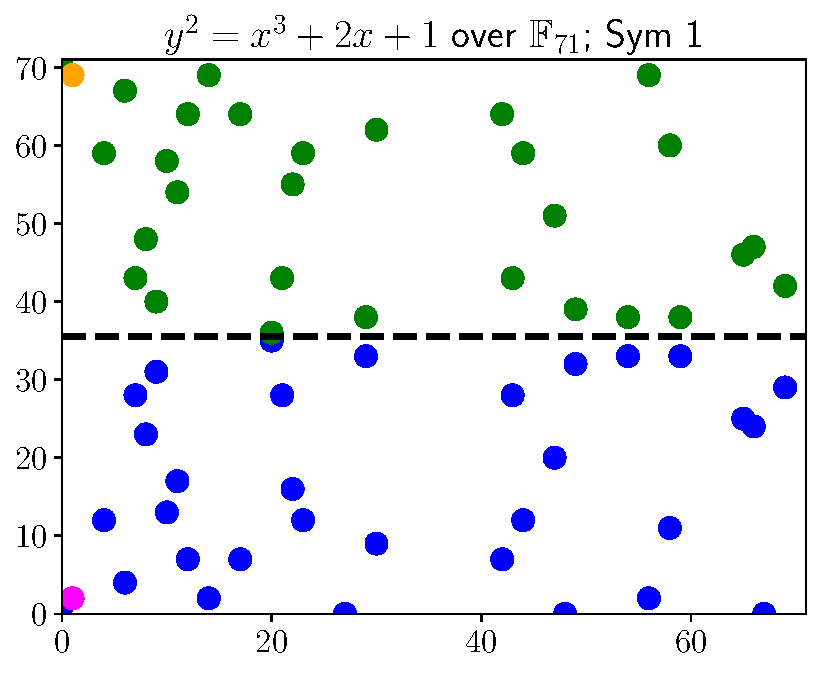
\includegraphics[width=\textwidth]{plots/ec_finite/ec_finite_F_71_2_1_symmetry_1.pdf}
    \caption{Plot with $y$ values in $\brackets{0,p}$.}
    \label{fig:ec_finite_plots_symmetry_1}
    \end{subfigure}
    \begin{subfigure}[t]{0.45\textwidth}
    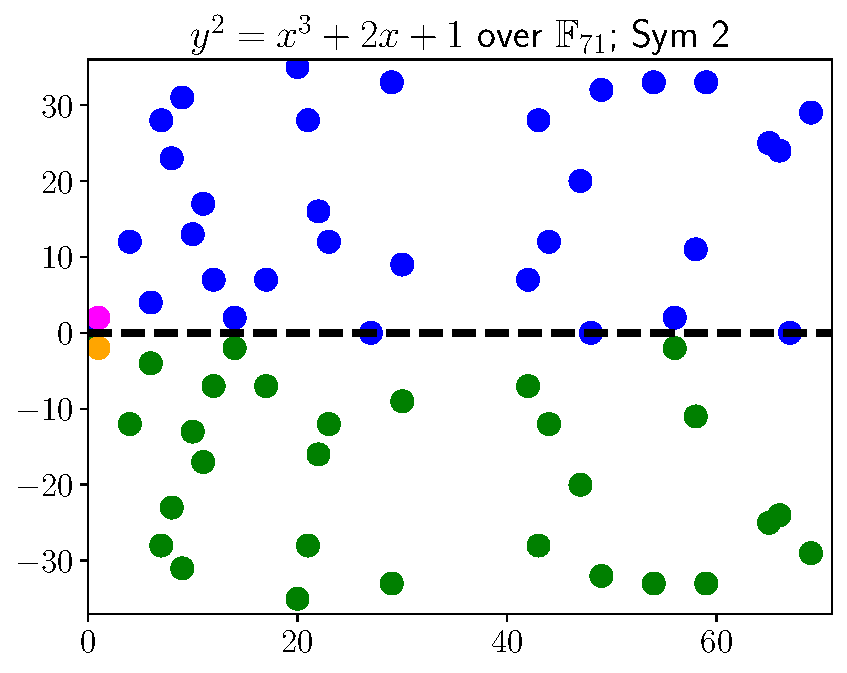
\includegraphics[width=\textwidth]{plots/ec_finite/ec_finite_F_71_2_1_symmetry_2.pdf}
    \caption{Plot with $y$ values in $\brackets{-p/2,p/2}$.}
    \label{fig:ec_finite_plots_symmetry_2}
    \end{subfigure}
\caption[Plots showing symmetry of elliptic curves over finite fields]{Here
    have a plot showing the symmetry of \glspl{elliptic curve} over $\F_{71}$.
    The ``positive'' points are in \textcolor{blue}{blue}
        with $y$-values between $0$ and $p/2$;
    the ``negative'' points are in \textcolor[rgb]{0,0.33,0}{green}
        with $y$-values between $p/2$ and $p$.
    Because $-y = p-y\mod p$,
    the negative points are equivalent to those with $y$ values
    between $-p/2$ and $0$.
    }
\label{fig:ec_finite_plots_symmetry}
\end{figure}
